\documentclass{article} 
\usepackage[a4paper]{geometry} 
\usepackage{graphicx} 
\usepackage{hyperref} 
\usepackage{amsmath,amssymb} 
\usepackage{caption} 
\usepackage{subcaption}
\usepackage{pdflscape}
\usepackage{listings}

\title{Searching for Supersymmetric Higgs Bosons} 
\author{ Daniel C E Bunting \& Amalia Madden} 
\date{\today}

\newcommand{\includecode}[2][c]{\lstinputlisting[caption=#2, escapechar=, style=custom#1]{#2}}


\begin{document}

\maketitle
\begin{abstract}
\end{abstract}

\section{Introduction} % (fold)
\label{sec:introduction}

% section introduction (end)

\section{Theory} % (fold)
\label{sec:theory}
%!TEX root = /Users/Daniel/Documents/Imperial/project/tevatron-higgs/report/report.tex
The standard model represents our current understanding of fundamental particles and their interactions. Its development stemmed from the discovery in the 1970s of a symmetry between the weak and electromagnetic forces which allowed them to be unified as a single force. The equations of this unified theory correctly described the electroweak force and its associated bosons, but with a serious issue that all emerged without mass. Whilst true for a photon, we know that the W and Z bosons have significant mass.

To solve this problem, a mechanism was proposed by theorists Robert Brout, François Englert and Peter Higgs, whereby particles are given mass through interaction with the Higgs field. Mass of a particle is dependent on the strength of its interaction with the field – for example photons do not interact with it at all. The particle associated with the fundamental Higgs field is the Higgs boson.

Observation of a new particle with a mass of 126 Gev was announced on 4 July 2012 by the ATLAS and CMS experiments at CERN's Large Hadron Collider. This particle is thought to be consistent with the Higgs Boson, and lead to the award of the Nobel prize in 2013 to François Englert and Peter Higgs.


Quantum field theories such as the standard model comprise two basic types of field, fermions that lead to matter particles and bosons that lead to force-carrier. The spin-statistics theorem asserts that these two types are differentiated in that bosons have integer spins and fermions half-odd-integer spins. The creation of a symmetry that relates fermions and bosons forms the basis supersymmetry, whose major proponent is the existence of a new set of partner particles to those in the standard model. The superpartners differ by a spin of a half, so that bosons will be partnered with fermions and vice-versa. 

The existence of these new particles could solve a major problem of fixing the mass of the Higgs Boson. The observed mass of the Higgs boson is puzzlingly light when interactions with the particles of the standard model should make it very heavy. The addition of the extra particles in supersymmetry could cancel out contributions to the Higgs mass from their Standard-Model partners. 

The minimal supersymmetric standard model (MSSM) investigated here is the supersymmetry model with the minimum number of new particle states and interactions that are consistent with phenomenology,. Whereas in the Standard Model the Higgs field is introduced as a weak isospin doublet, in the
MSSM the presence of two of these doublets leads to five physical Higgs bosons, three neutral (collectively denoted as $\phi$): h, H, and A ; and two charged: $H^-$ and $H^+$.

To describe the MSSM Higgs model, two free parameters are conventionally chosen - $\tan\beta$, the ratio of the vacuum expectation values of the two Higgs doublets, and the mass of A, one of the MSSM Higgs. Although $\tan\beta$ is a free parameter in MSSM, a large value of $\tan\beta \approx 35$ would explain the ratio of the top to bottom quark mass, and also provide good reason for the observed density of dark matter.

The value of $\tan\beta$ provides an enhancement factor for the couplings of the Higgs to fermions in the SM compared to the MSSM. The couplings of the Higgs in the MSSM are proportional to those in the SM and depend also on the type of quark and Higgs. For large $\tan\beta$, two of the Higgs Bosons A and either h or H have approximately the same mass. Whilst their coupling to down-type quarks is enhanced by $\tan\beta$ compared to the SM, their coupling to up-type quarks is reduced.  Due to this enhancement, the most probable mode of decay for the three neutral Higgs bosons is $\phi  \rightarrow b\bar{b} $  with a branching ratio near 90\% (the next most probable being 
$\phi  \rightarrow \tau\bar{\tau} $ ). Due to large multijet backgrounds a direct search for $\phi \rightarrow b\bar{b} $ is difficult. Instead, the case $\phi b \rightarrow b\bar{b}b $ where $\phi$ is produced in association with one b quark is used which.



% section theory (end)


\section{Method} % (fold)
\label{sec:method}

\subsection{Event Simulation} % (fold)
\label{sub:event_simulation}
%!TEX root = /Users/Daniel/Documents/Imperial/project/tevatron-higgs/report/report.tex

The Monte Carlo simulation of the events used in the training and evaluation of the neural networks is beyond the scope of this project, so will only be briefly summarised here. Signal $\phi b \rightarrow b\bar{b}b $ events were simulated using the PYTHIA event generator \cite{sjostrand2006pythia} to leading order, with a mass hypothesis  of $M_H = 110 \mathrm{GeV/c^2}$ and then corrected to next-to-leading order with MCFM \cite{campbell2010mcfm}. 
The background multijet events were generated using ALPGEN \cite{mangano2003alpgen}. The simulated events were then passed through a model of the D$\emptyset$ detector \cite{brun1993geant}.
Finally various preprocessing cuts were applied to the data excluding unlikely signal events, giving a final total of 53,960 events.


\begin{figure}[htbp]
	\centering
		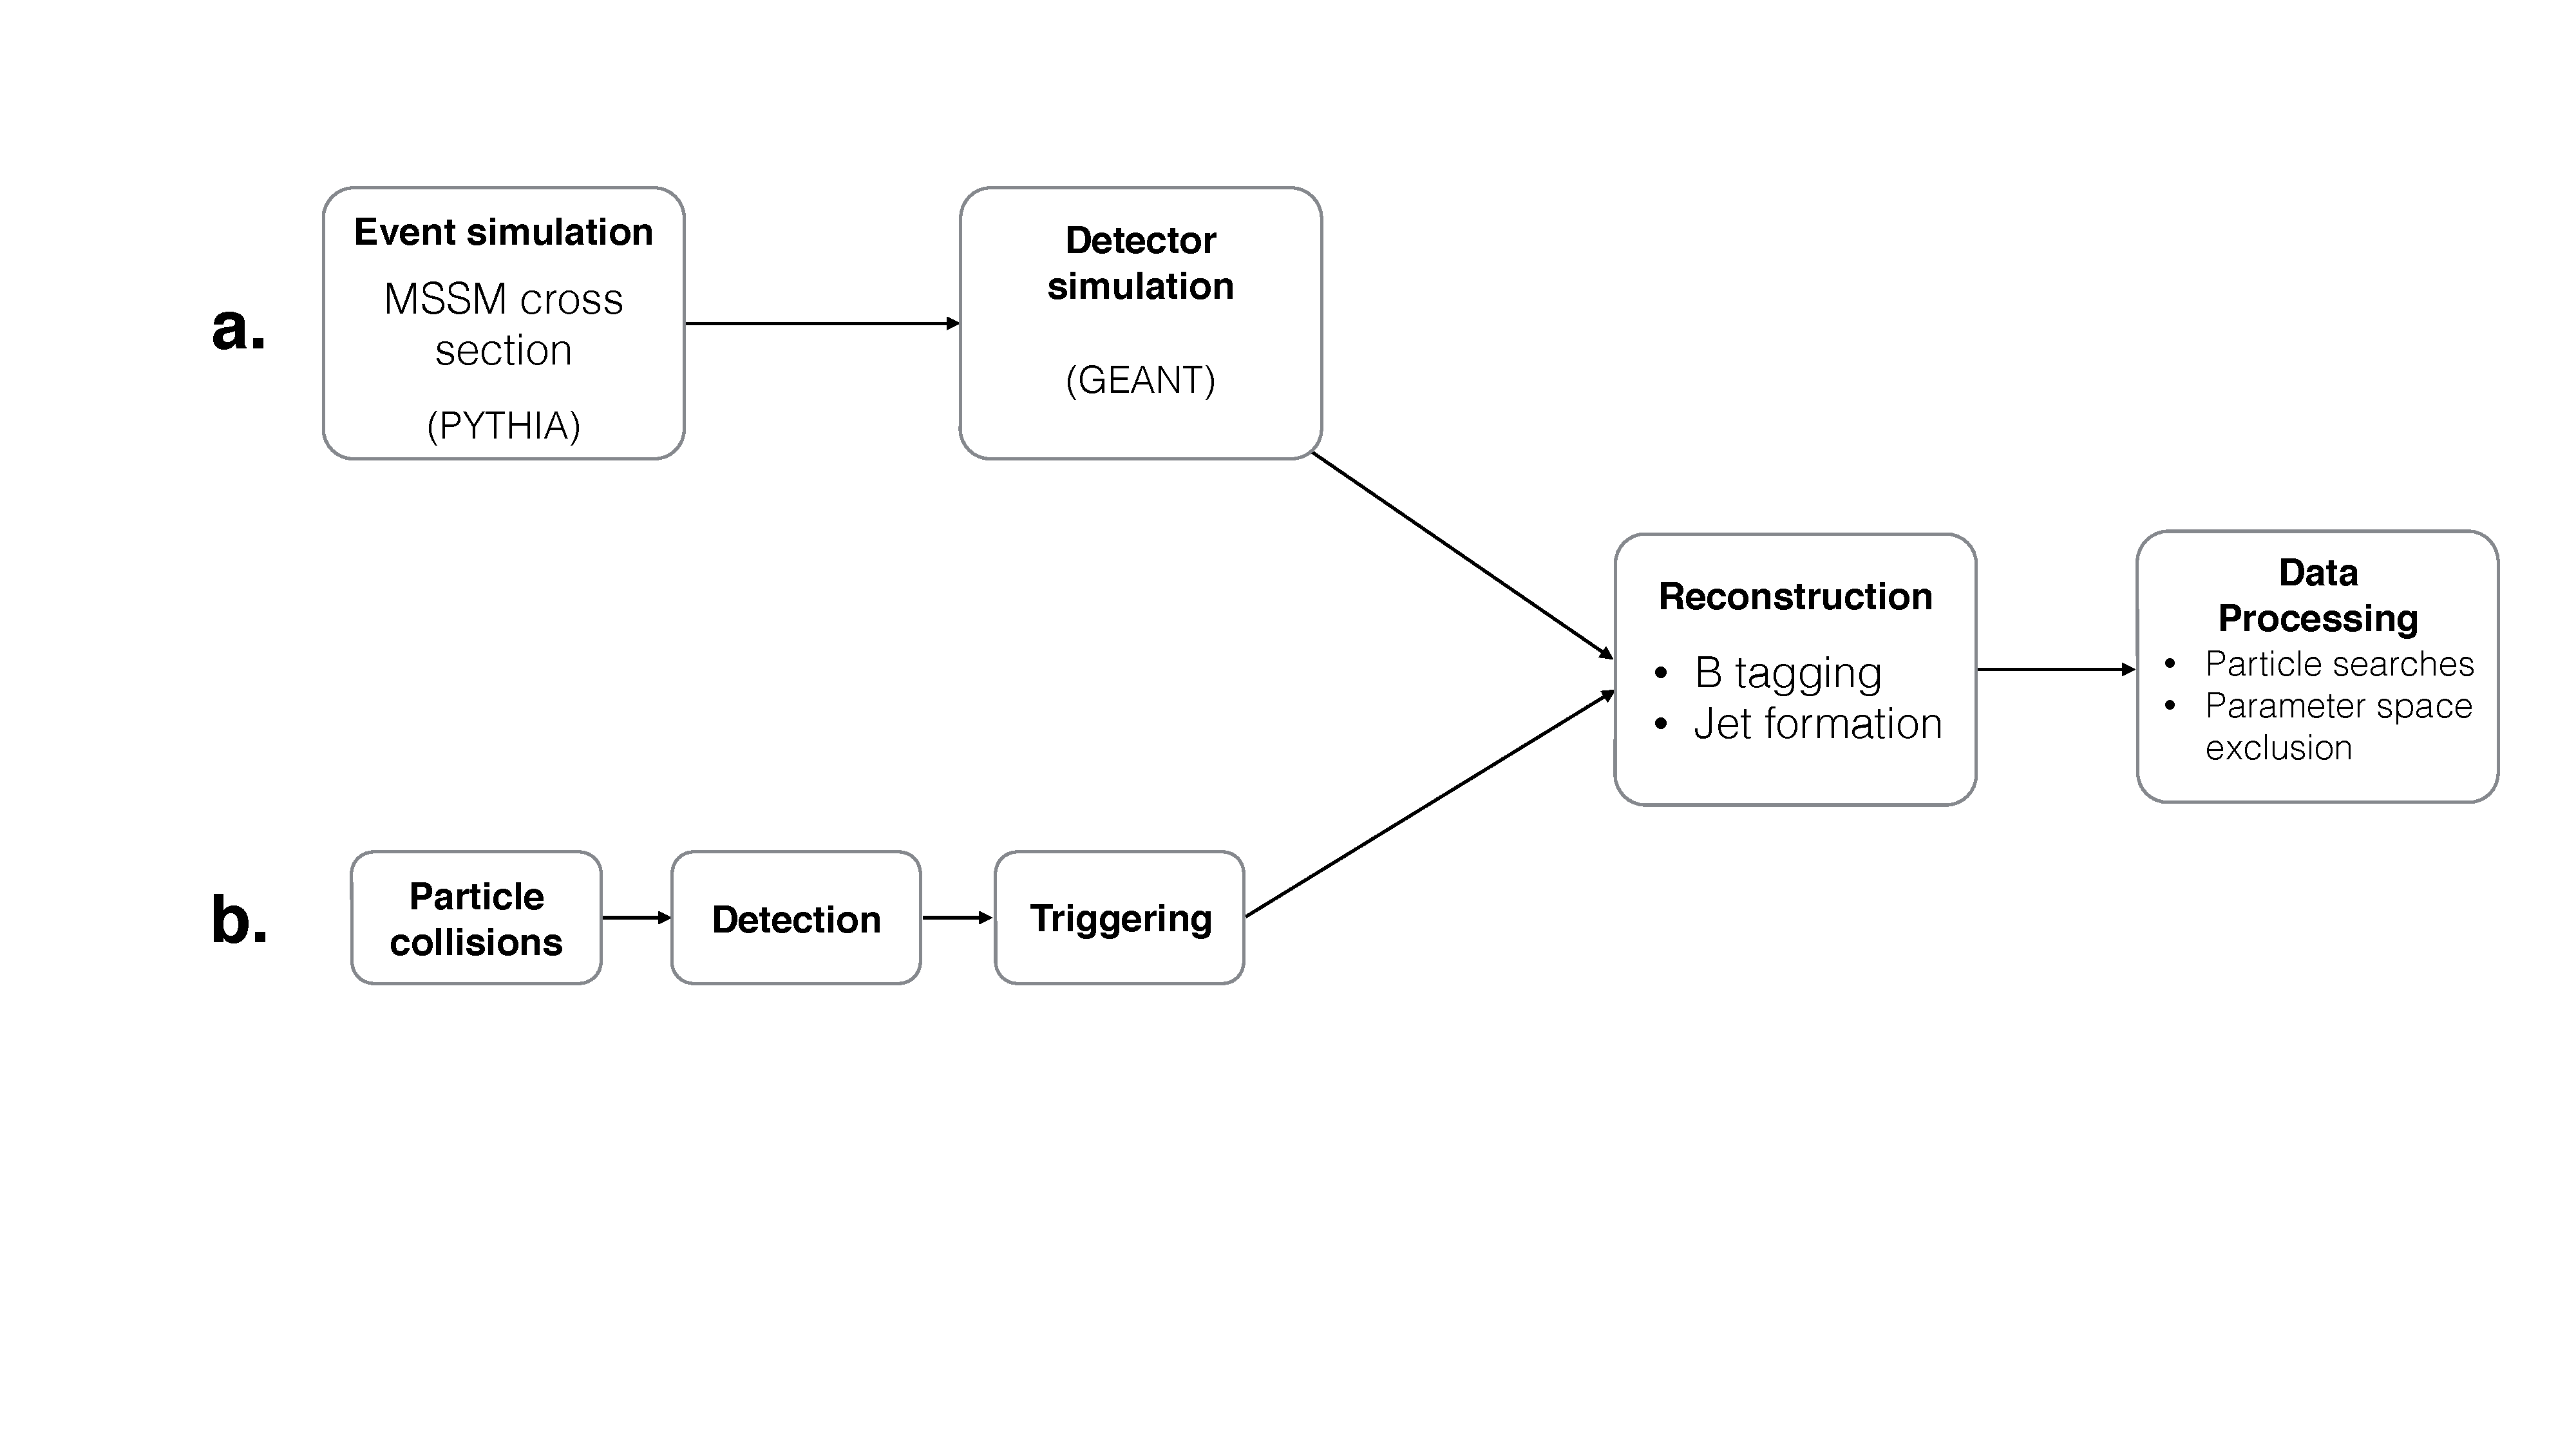
\includegraphics[width=\textwidth]{img/flow}
	\caption{Steps in the information processing pipeline for a. simulated and b. measured data.  }
	\label{fig:flow}
\end{figure}
% subsection event_simulation (end)

\subsection{Feature Selection} % (fold)
\label{sub:feature_selection}
%!TEX root = /Users/Daniel/Documents/Imperial/project/tevatron-higgs/report/report.tex

In any scenario where statistical methods are used to interpret data selecting features in order to maximise the discriminatory or explanatory power of the model plays a critical role.
From the b-tagged jets, those with the highest and second highest transverse momentum $P_t$ were identified as being the putative product of the decaying Higgs boson, with all the following variable differences are considered to be taken between these leading jets. 
Following \cite{Abazov201197} seven feature variables were extracted from the raw simulation data, and used as inputs to the classification neural network. 

\subsubsection*{Pseudorapidity difference $ \Delta\eta $ } % (fold)
\label{ssub:pseudorapidity}

Te pseudorapidity of a jet is defined as
\begin{equation}
	\eta = - \ln\left[\tan\left( \frac{\theta}{2} \right)\right]
\end{equation}
where $\theta$ is the angle between the jet and the beam axis. The pseudorapidity is preferred to $\theta$ as the difference between two pseudorapidity is Lorentz invariant.
% subsubsection pseudorapidity (end)


\subsubsection*{Momentum balance $P_{balance}$} % (fold)
\label{ssub:momentum_balance_p__balance}

The momentum balance of the leading b jet pair is defined

\begin{equation}
	P_{balance} = \frac{\left|p_1 - p_2\right|}{ \left|p_1 + p_2\right|}  
\end{equation}

% subsubsection momentum_balance_p__balance (end)

\subsubsection*{Sphericity $S$} % (fold)
\label{ssub:sphericity_s}
	The sphericity is defined as 
	\begin{equation}
		S = \frac{3}{2} (\lambda_2 + \lambda_3)
	\end{equation}

	where $\lambda_2$ and $\lambda_3$ are the second and third largest eigenvalues of the sphericity tensor $\mathbf{\hat{S}}^{\alpha\beta}$
	\begin{equation}
		\mathbf{\hat{S}}^{\alpha\beta} = \frac{\sum_i p_{\alpha}^i p_{\beta}^i}{\sum_i |p^i|^2}
	\end{equation}

% subsubsection sphericity_s (end)

\subsubsection{Invariant Mass} % (fold)
\label{ssub:invariant_mass}

\begin{equation}
	M_H = \sqrt{\sum_{Dijet}{E^2 - p^2}}
\end{equation}

As can be seen in Table~\ref{tab:corr} the invariant dijet mass is a strong predictor of whether an event is Higgs decay and including it in the ANN significantly increased its discriminatory power.
However since the Higgs mass is not predicted by the Standard Model it must be hypothesised during the simulation stage, so in order to avoid training the ANN to depend too heavily on a particular value of $M_H$ we tested models both with and without $M_H$
% subsubsection invariant_mass (end)


Additionally we define the \textbf{azimuthal angle difference $ \Delta\phi $}, the \textbf{combined pseudorapidity $\eta_H$}, the \textbf{difference between the leading jet and the Higgs $\eta_H - \eta_1$}.

\begin{figure}[htbp]
	\centering
	\begin{subfigure}[b]{0.395\textwidth}
		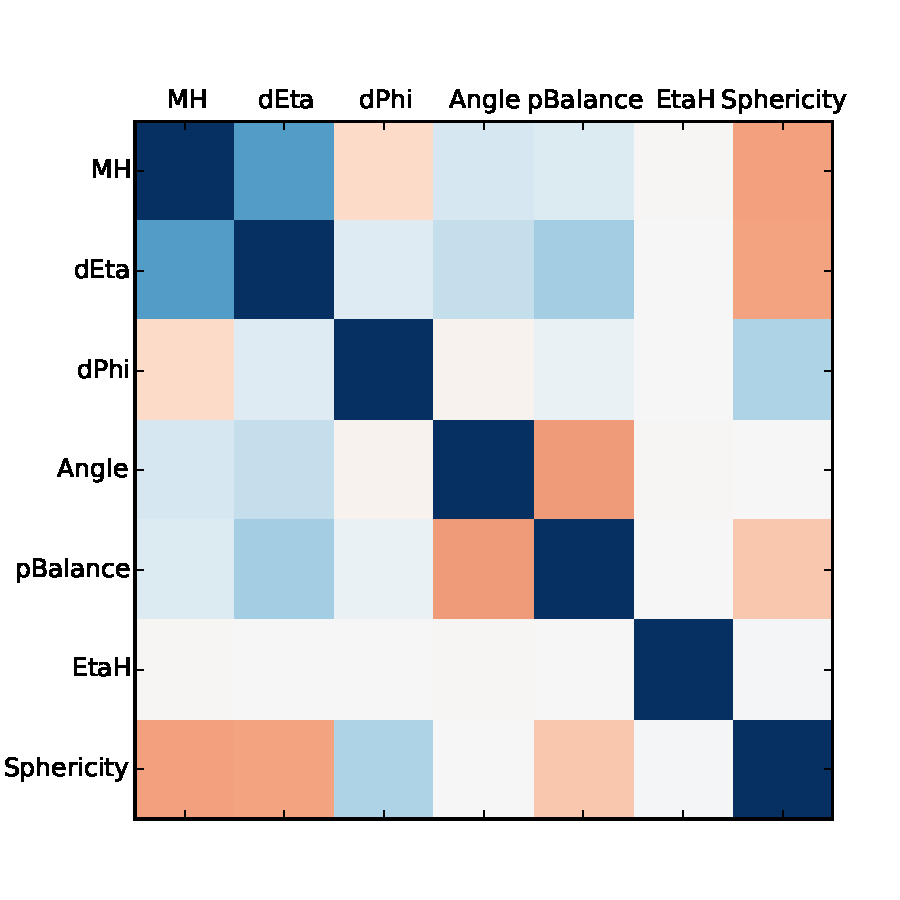
\includegraphics[width=\textwidth]{img/background_corr}
		\caption{Background}
		\label{fig:mh}
		\vspace{7mm}
	\end{subfigure}
	\begin{subfigure}[b]{0.5\textwidth}
		                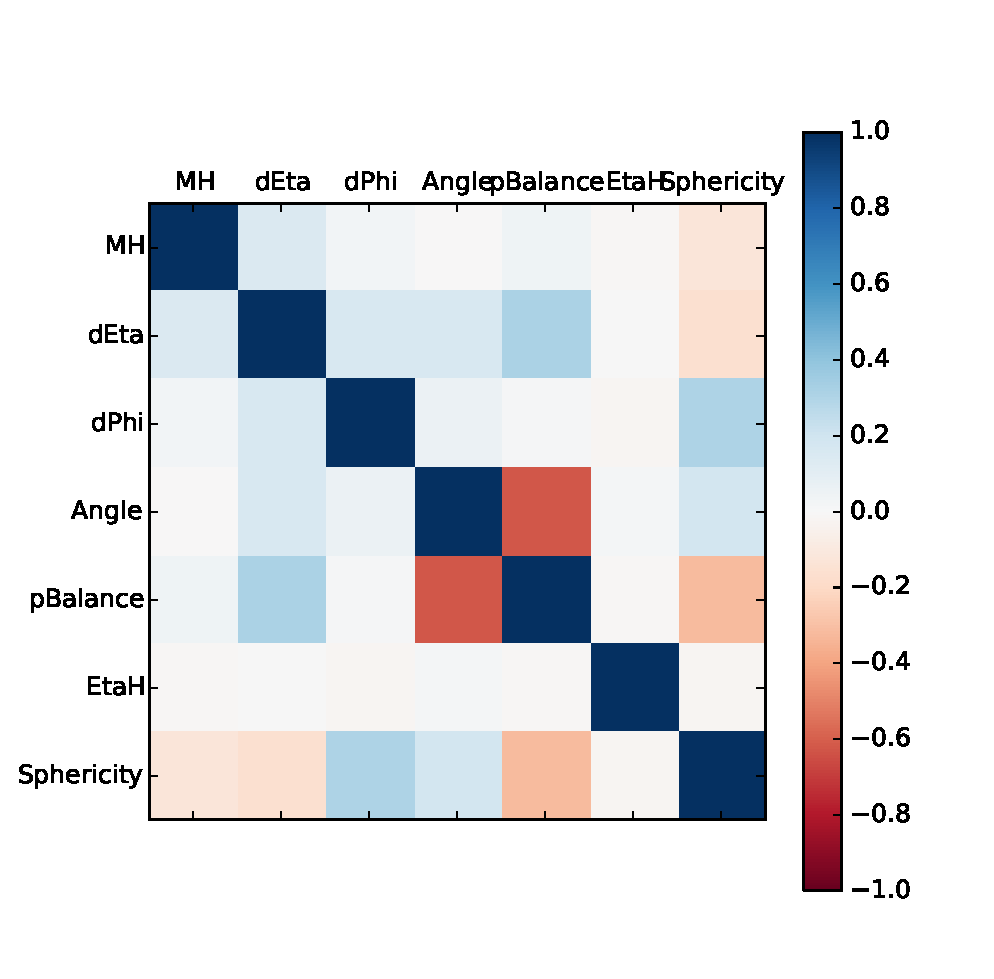
\includegraphics[width=\textwidth]{img/signal_corr}
		                \caption{Signal}
		                \label{fig:mh}
		\end{subfigure}
	
	\caption{Matrices of the Pearson product-moment correlation coefficients between each of the features}
	\label{fig:cormat}
	\end{figure} 

	
In order to evaluate the the feature selection the correlation matrices between the features for the signal and background events were calculated and shown in Figure~\ref{fig:cormat}. 
The correlations between each feature and the output variable were also calculated and are summarised in  Table~\ref{tab:corr}. 
The features selected for inclusion in a model should be both highly correlated with the output and weakly correlated with each other. A high correlation between two features suggests redundancy, which should be avoided as unnecessarily complex models take longer and require more data (which may not be available) to train.
$\eta_{H}$ is a potential candidate for removal since it is very weakly correlated with the output.  
	\begin{table}
		\begin{center}
		\begin{tabular}{ll}
			\textbf{Feature} & \textbf{Correlation} \\
			\hline
			$\Delta\eta$ & 0.329\\			
			$M_{H}$ & 0.204 \\
			$\Delta\Phi$ &  0.176\\
			Sphericity & 0.150\\
			Momentum Balance &  0.134\\
			$\eta_H - \eta_1$ &  0.0343 \\
			$\eta_{H}$ & 0.00359\\
			
		\end{tabular}
		\end{center}
		\caption{The correlation between each of the features and the output variable}
		\label{tab:corr}
	\end{table}
	

\begin{figure}[htbp]
	\centering	
	\begin{subfigure}[b]{0.3\textwidth}
	                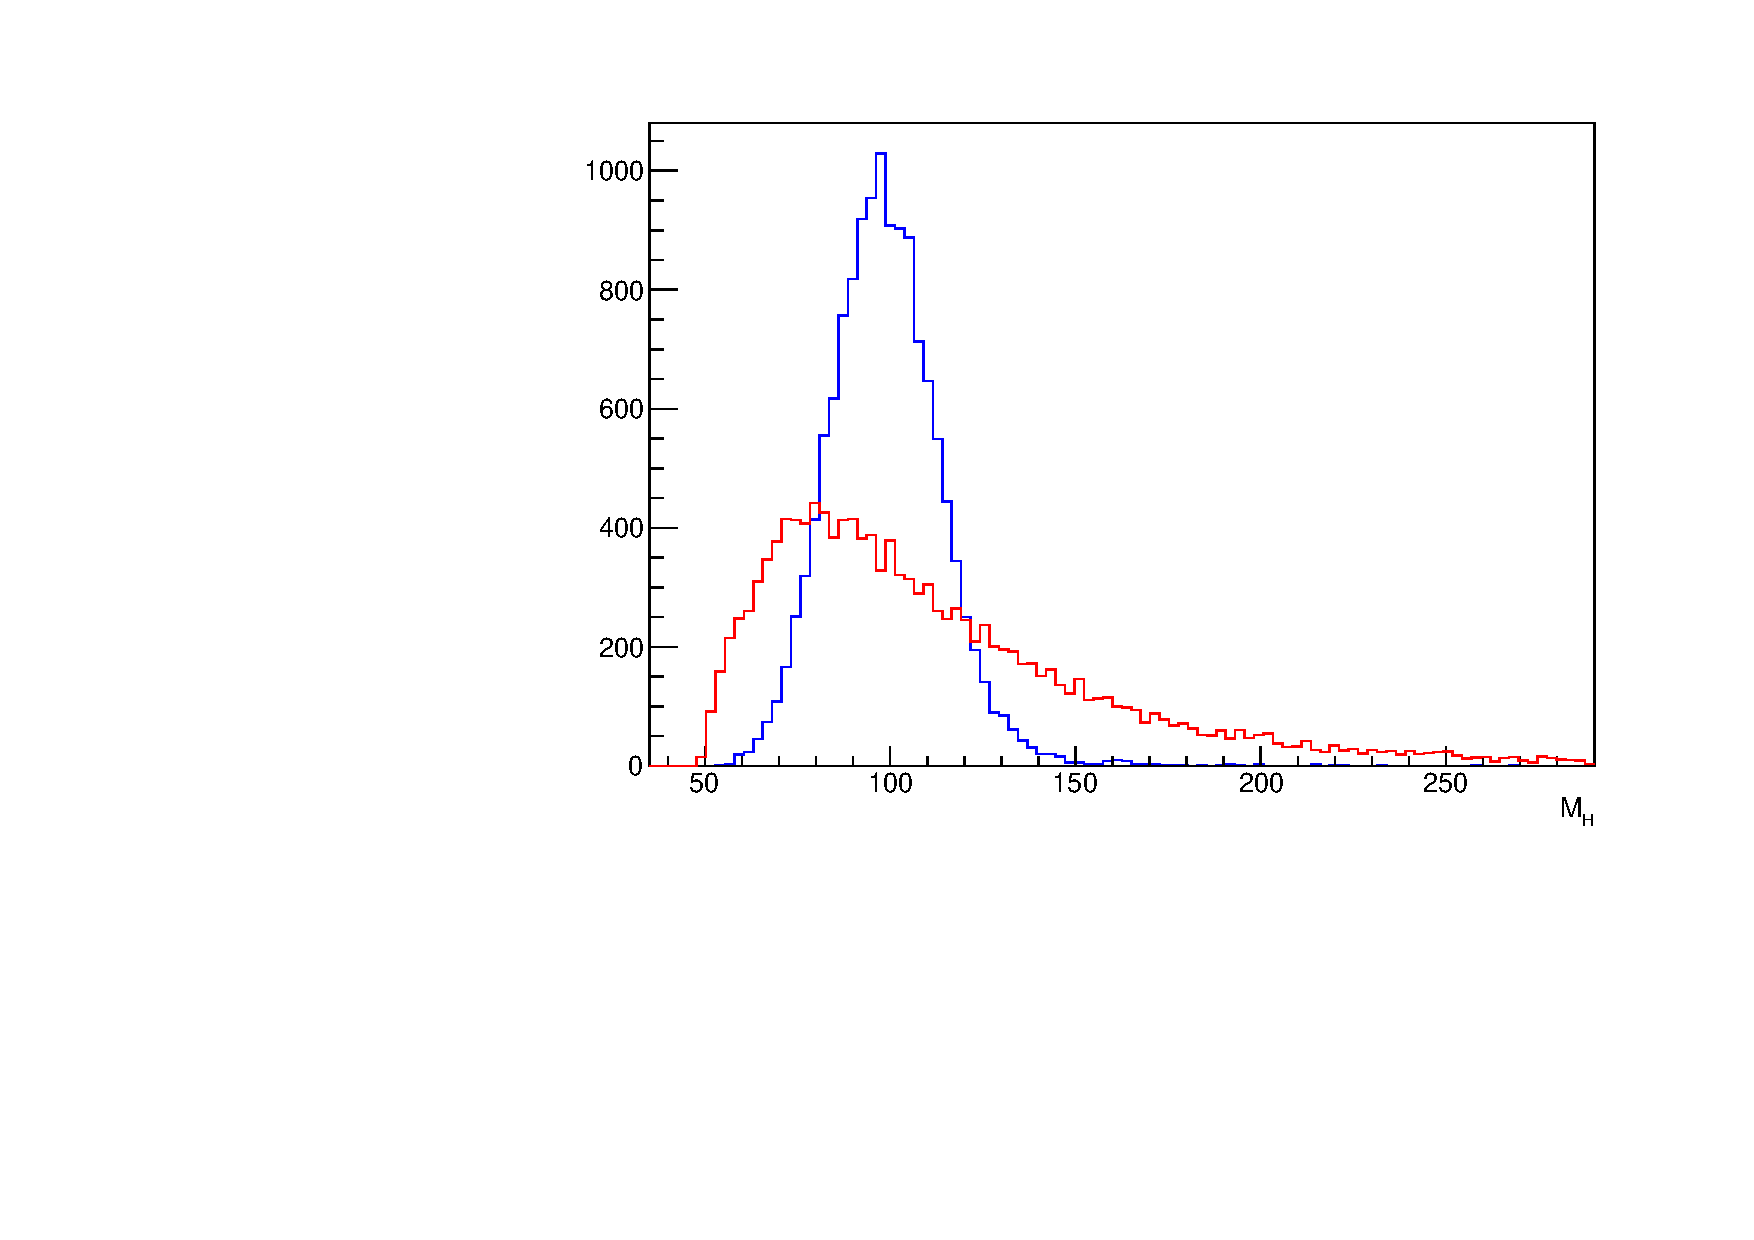
\includegraphics[width=\textwidth]{img/mh}
	                \caption{Invariant mass}
	                \label{fig:mh}
	\end{subfigure}
	\begin{subfigure}[b]{0.3\textwidth}
	                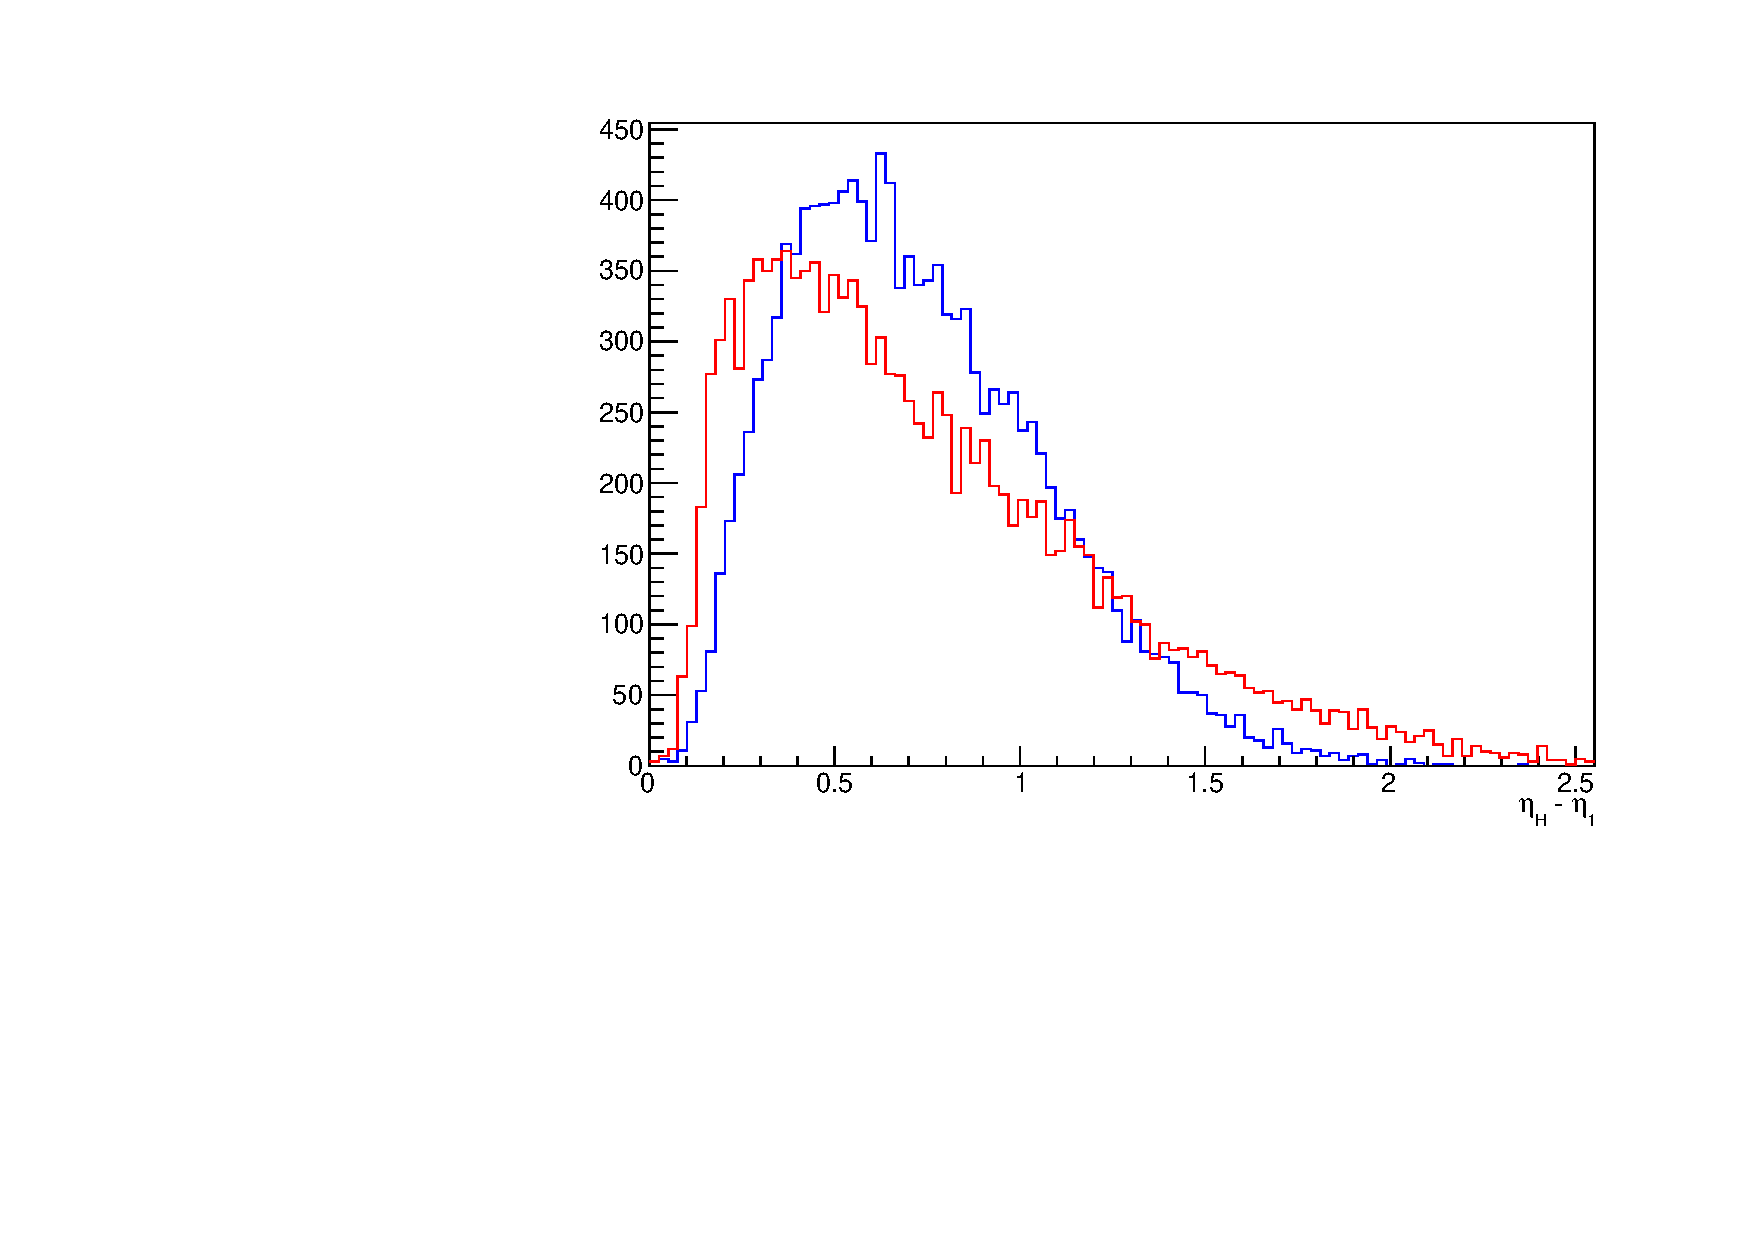
\includegraphics[width=\textwidth]{img/angle}
	                \caption{$\eta_H - \eta_1$}
	                \label{fig:angle}
	\end{subfigure}
	\begin{subfigure}[b]{0.3\textwidth}
	                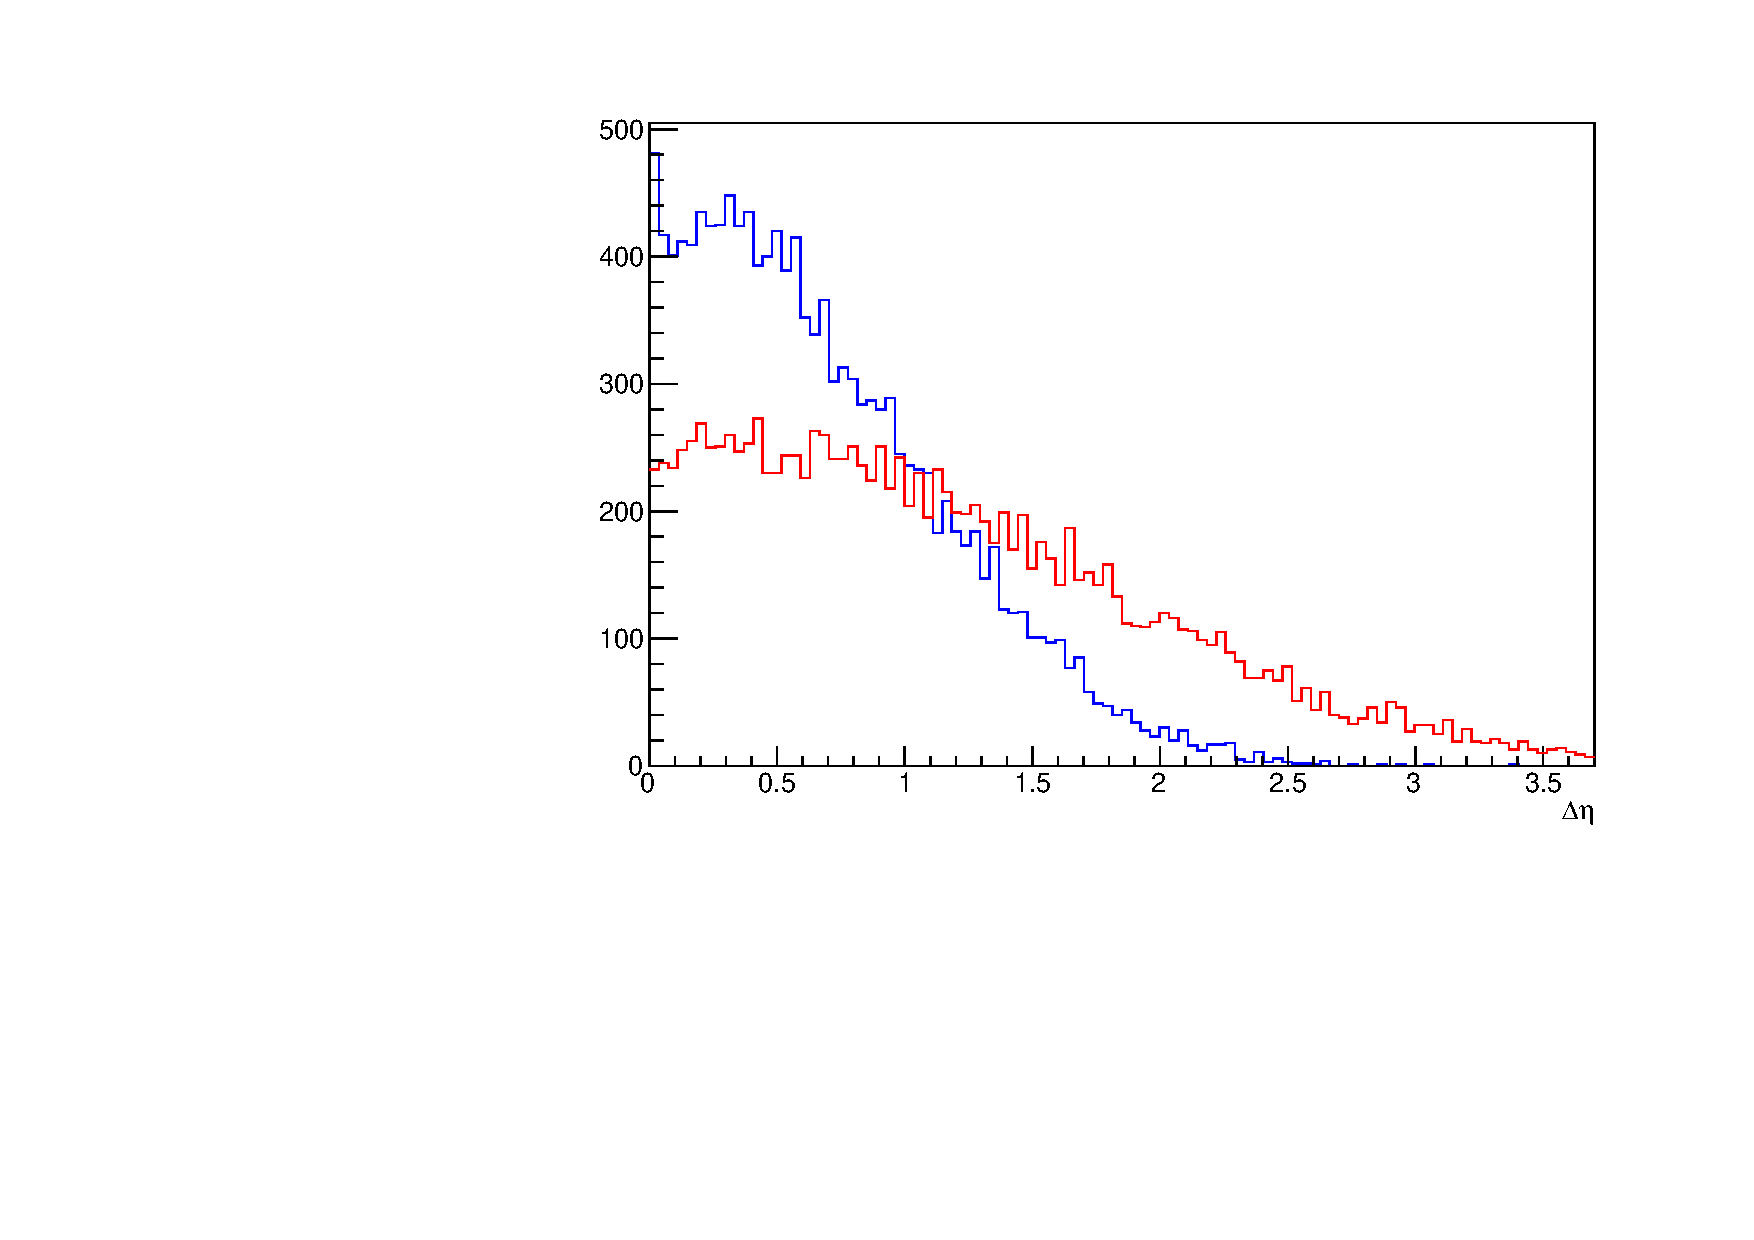
\includegraphics[width=\textwidth]{img/deta}
	                \caption{$\Delta\eta$}
	                \label{fig:deta}
	\end{subfigure}
	\begin{subfigure}[b]{0.3\textwidth}
	                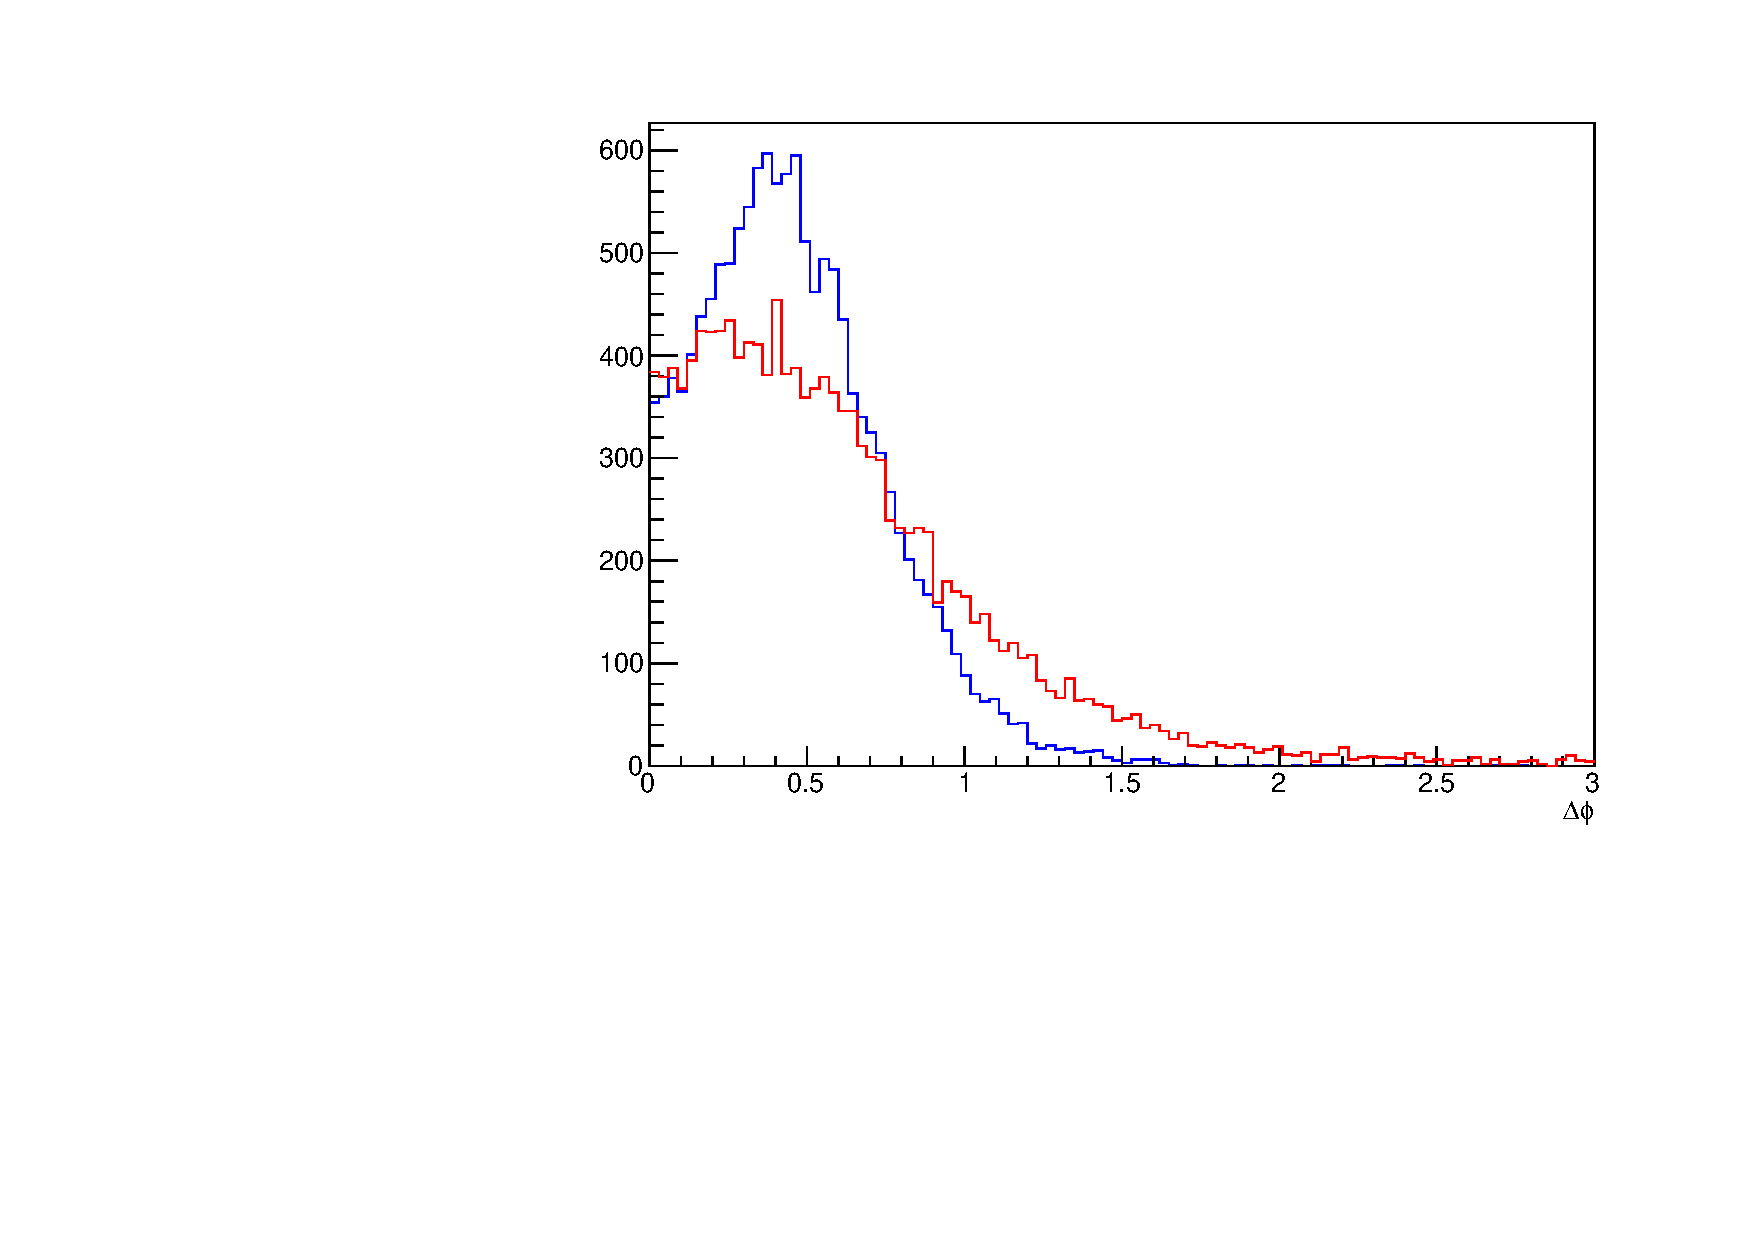
\includegraphics[width=\textwidth]{img/dphi}
	                \caption{$\Delta\phi$}
	                \label{fig:dphi}
	\end{subfigure}	
	\begin{subfigure}[b]{0.3\textwidth}
	                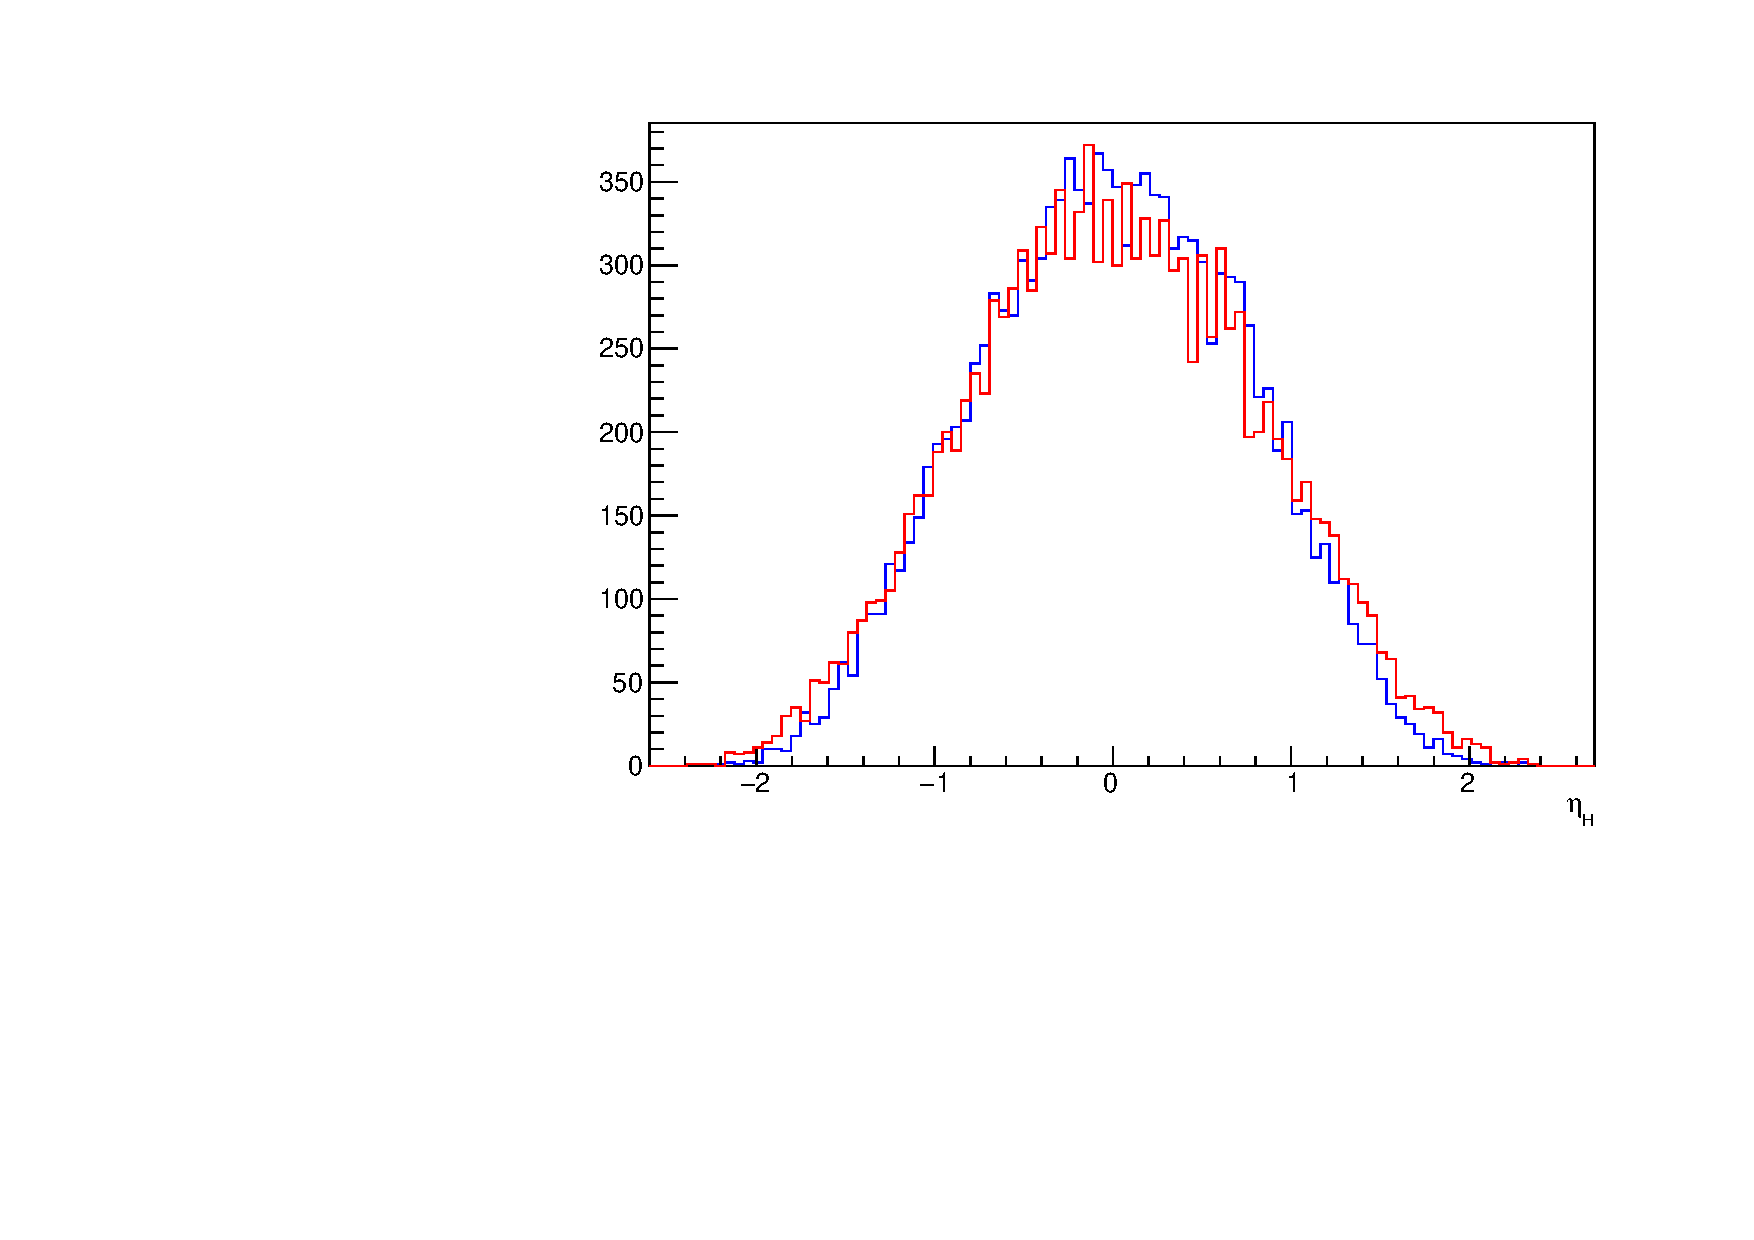
\includegraphics[width=\textwidth]{img/etah}
	                \caption{$\eta_H$}
	                \label{fig:etah}
	\end{subfigure}
	\begin{subfigure}[b]{0.3\textwidth}
	                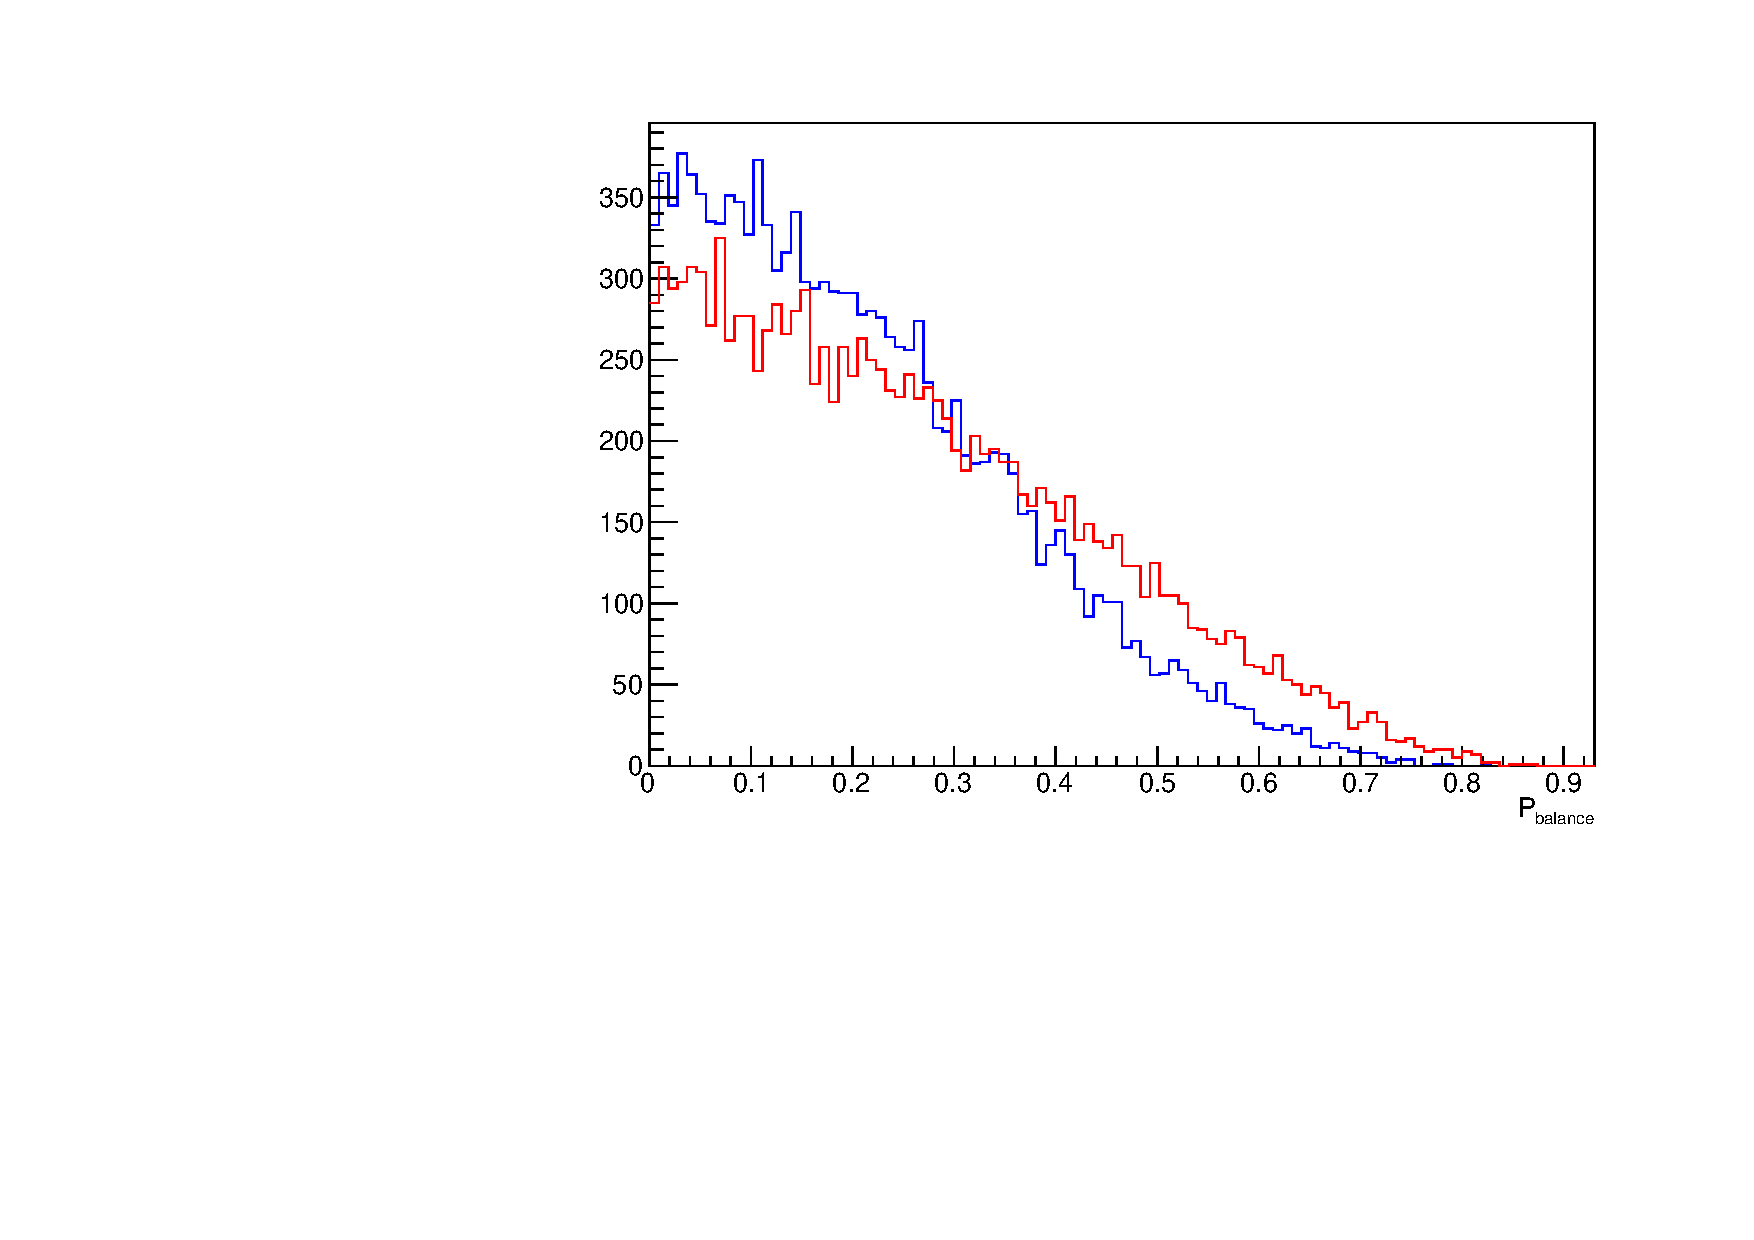
\includegraphics[width=\textwidth]{img/pbalance}
	                \caption{Momentum balance}
	                \label{fig:pbal}
	\end{subfigure}
	\begin{subfigure}[b]{0.3\textwidth}
	                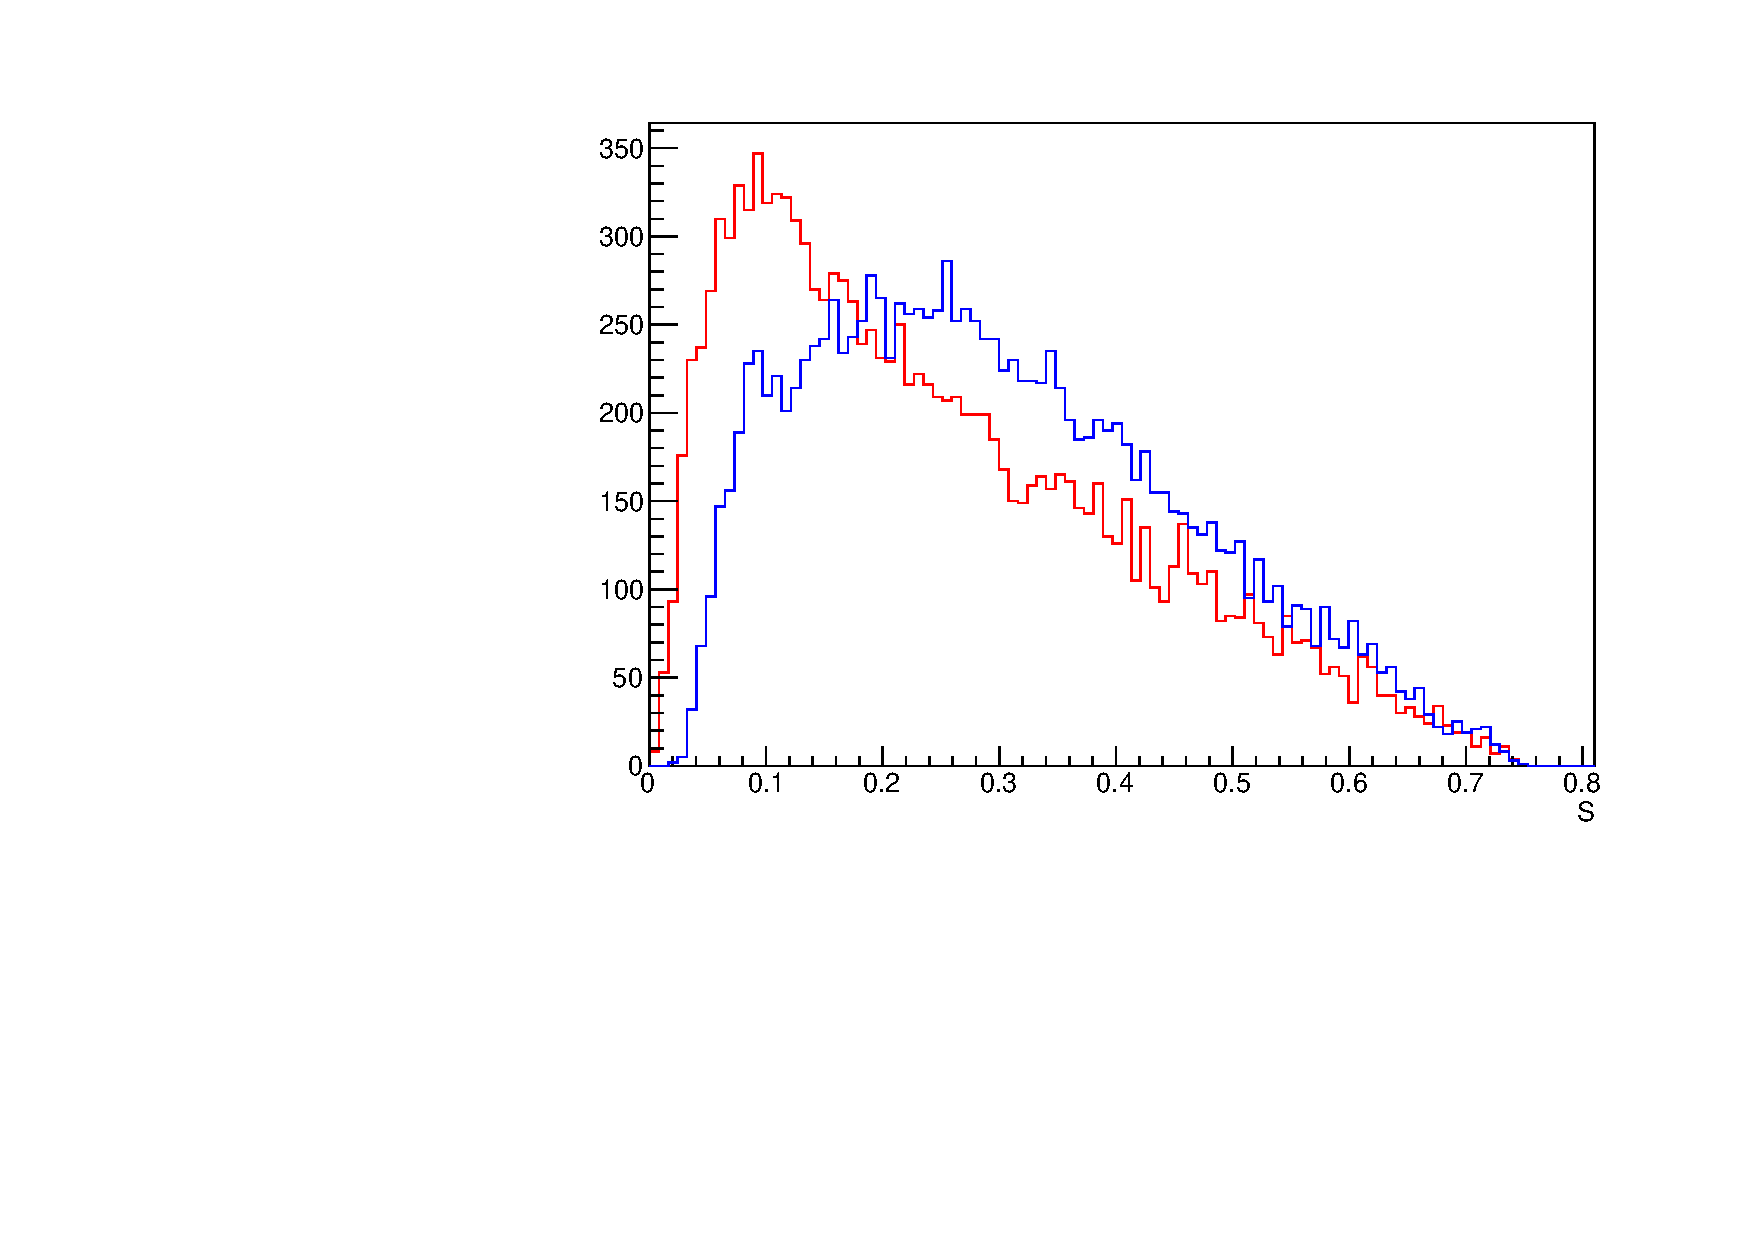
\includegraphics[width=\textwidth]{img/sphericity}
	                \caption{Sphericity}
	                \label{fig:sphericity}
	\end{subfigure}

	\caption{Distributions of the input features. All y scales are events. The signal is in blue and the background in red.}
	
	\label{fig:label}



\end{figure}


% subsection feature_selection (end)
\subsection{Artificial Neural Networks} % (fold)
\label{sub:artificial_neural_networks}


Heloo this is a test
% subsection artificial_neural_networks (end)

\subsubsection{Model Selection} % (fold)
\label{ssub:model_selection}
%!TEX root = /Users/Daniel/Documents/Imperial/project/tevatron-higgs/report/report.tex

The performance of a neural network is highly dependent on both the number of nodes and the network topology. 
In theory by the Universal Approximation Theorem, an ANN with sufficiently many nodes arranged in single hidden layer is able to approximate an arbitrary decision boundary. However in practice deep neural networks can perform better, so a variety of sizes and topologies were investigated and evaluated. 

A commonly used criterion for measuring signal/background separation performance is the significance, $\frac{S(c)}{\sqrt{B(c)}}$ where $S(c)$ and $B(c)$ are the weighted number of signal and background events respectively, scoring above the signal acceptance cutoff $c$. Typically,  as a function of $ c \in (0,1)$, $\frac{S(c)}{\sqrt{B(c)}}$ has a maximum which can be used as a comparison.

Another evaluation parameter common in machine learning applications is the AUC, the area under the ROC (receiver operator characteristic) curve.
The ROC curve is the parametric plot of the true positive rate (tpr) against the false positive rate (fpr), parameterised by the cutoff.

\begin{figure}[h]
	\centering
	
	\begin{subfigure}{0.49\textwidth}
	      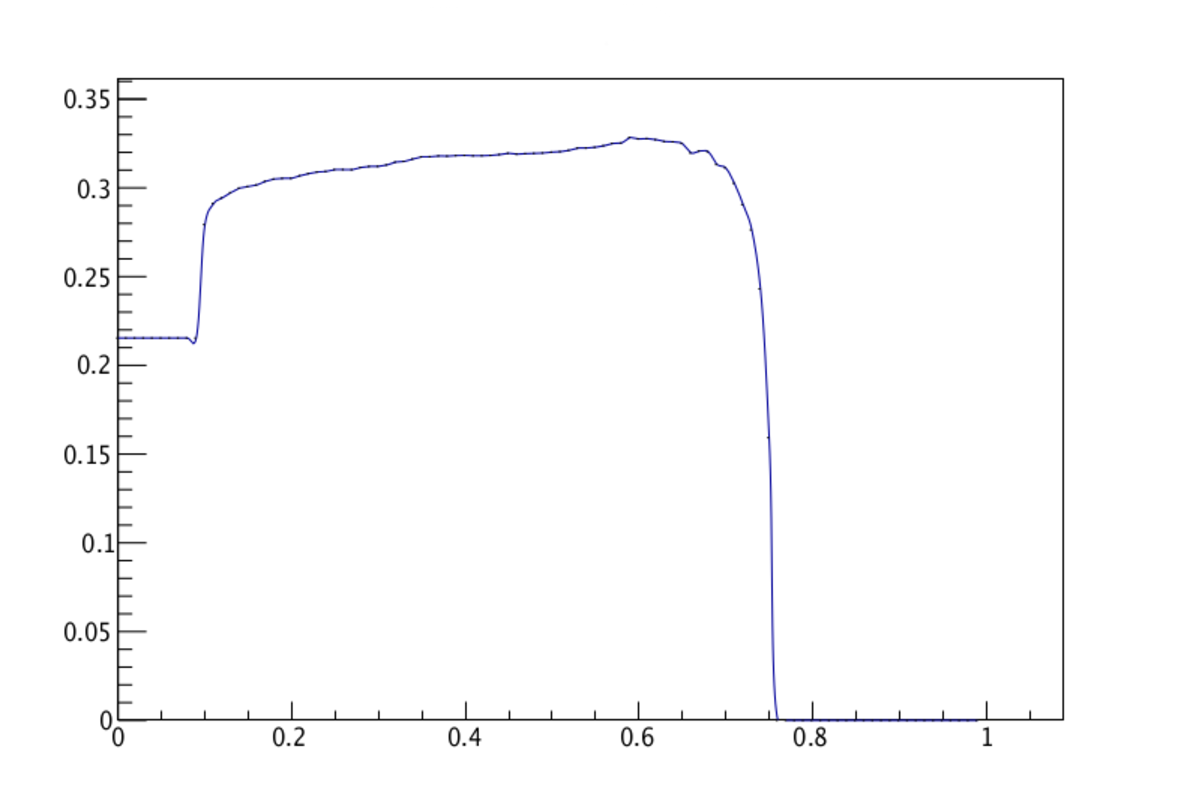
\includegraphics[width=\textwidth]{img/sig}
	      \caption{$\frac{S}{\sqrt{B}}$}
	\end{subfigure}
	\begin{subfigure}{0.49\textwidth}
	      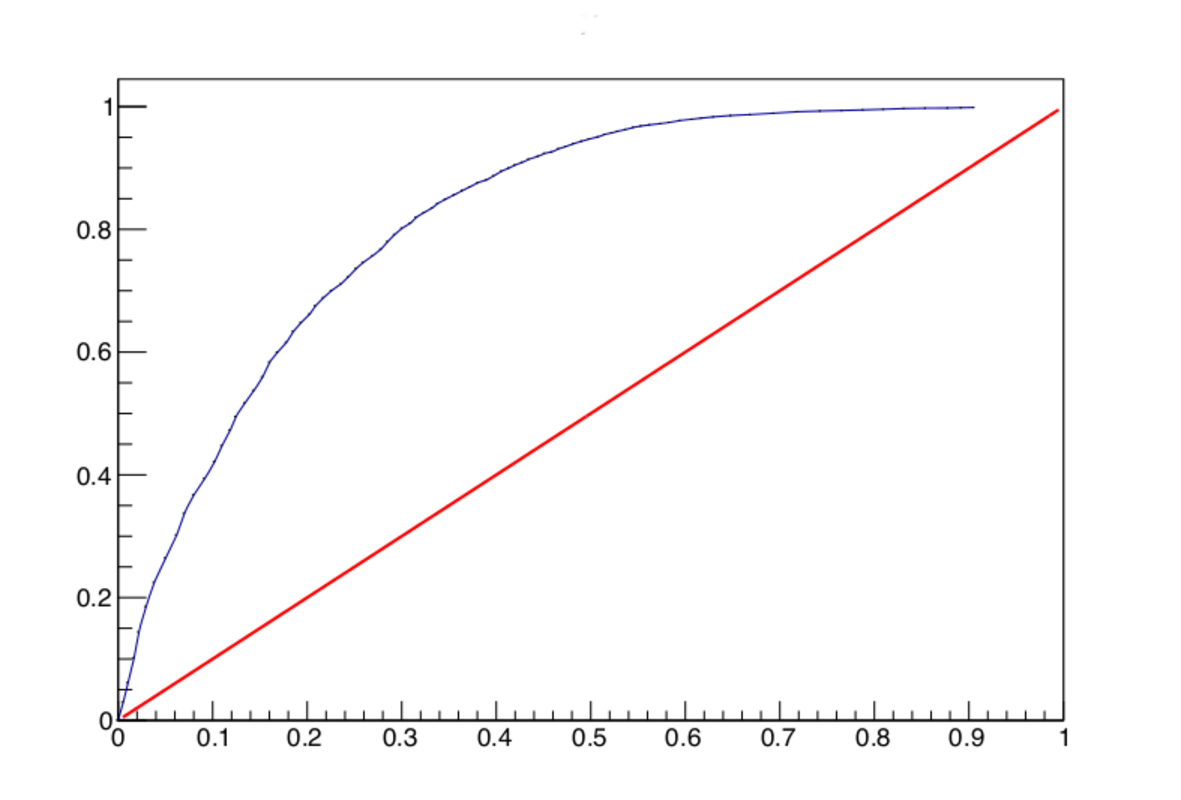
\includegraphics[width=\textwidth]{img/roc}
	      \caption{ROC curve of the classifier}
	\end{subfigure}
	
	\begin{subfigure}{0.5\textwidth}
	      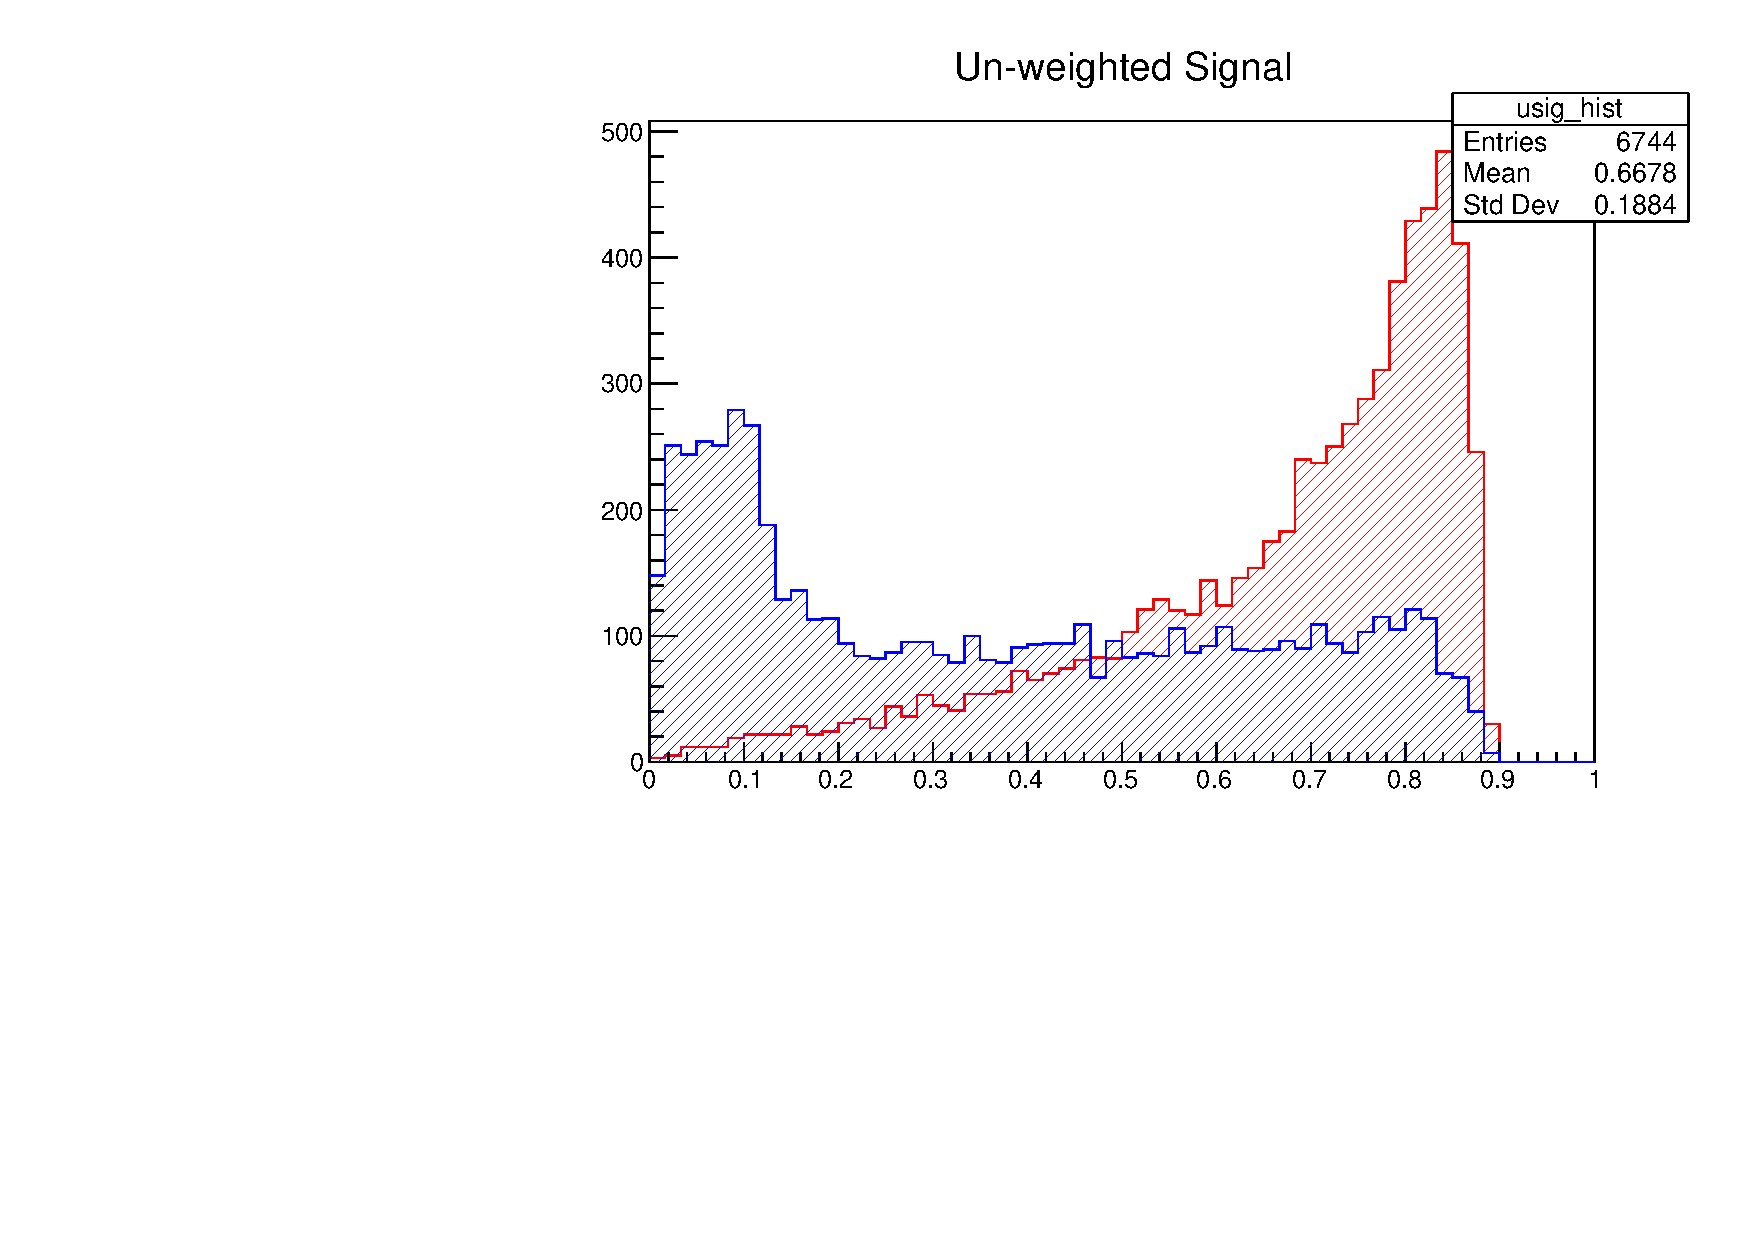
\includegraphics[width=\textwidth]{img/sep}
	      \caption{Distribution of model scores for signal (red) and background (blue) events}
	\end{subfigure}

	\caption{Diagnostic plots for a train ANN with two layers of seven and six hidden nodes }
	\label{fig:label}
\end{figure}

In order to evaluate the reliance of the network on the (hypothesised) invariant dijet mass, the network was trained and evaluated both with and without $M_H$ over single layer configurations with between 1 and 50 hidden nodes.
As expected Figure~\ref{fig:mhcomp} shows that removing $M_H$ as a feature had a significant negative effect on the accuracy of the network.

\begin{figure}[htbp]
	\centering
	\begin{subfigure}{0.49\textwidth}
	      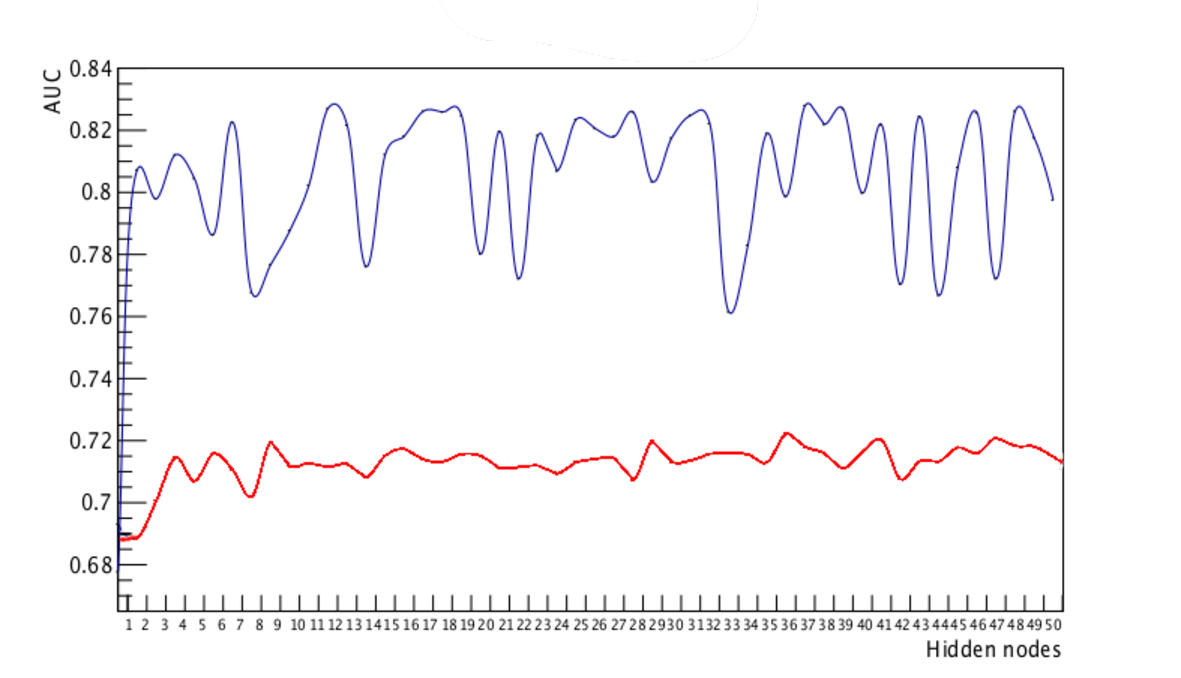
\includegraphics[width=\textwidth]{img/auc_1}
	      \caption{Area under ROC curve (AUC)}
	\end{subfigure}
	\begin{subfigure}{0.49\textwidth}
		  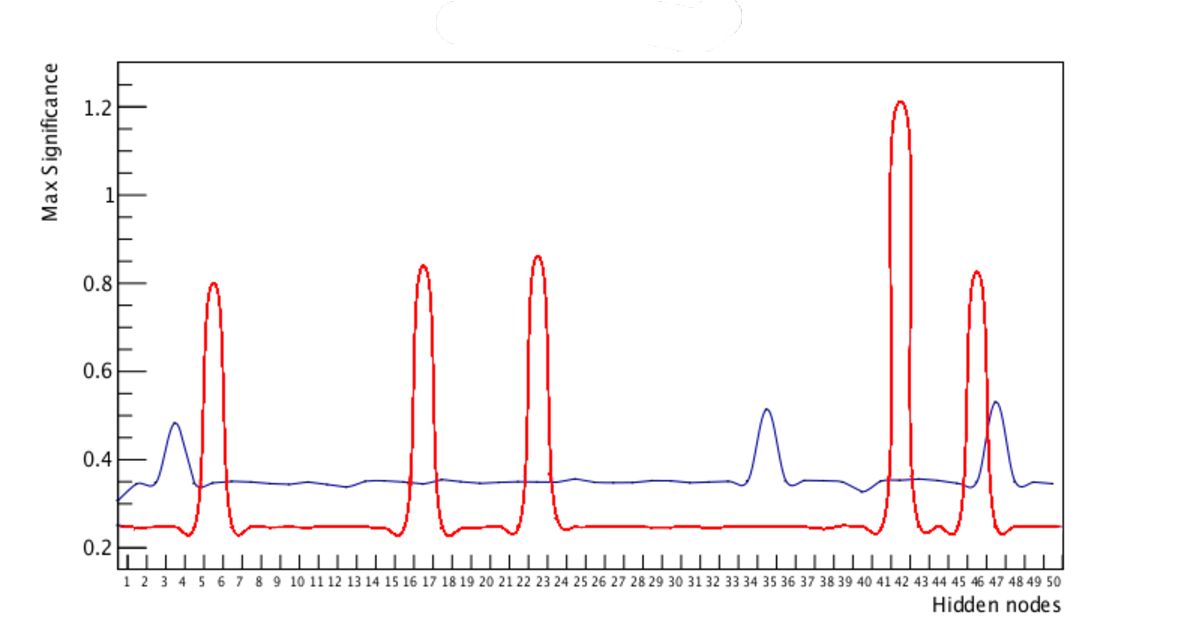
\includegraphics[width=\textwidth]{img/sig_1}
		  \caption{Maximum significance}
	\end{subfigure}
	\caption{The ANN evaluated with (blue) and without (red) the invariant dijet mass $M_H$ as a feature }
	\label{fig:mhcomp}
\end{figure}

We also considered the effect of a second hidden layer on the discriminatory power of the ANN
% subsubsection model_selection (end)


% section method (end)



\section{Conclusion} % (fold)
\label{sec:conclusion}
%!TEX root = /Users/Daniel/Documents/Imperial/project/tevatron-higgs/report/report.tex

In this project artificial neural networks were used to identify Higgs boson decay events in the $b\bar{b}b$ channel for the purpose of identifying the excess of $\phi \rightarrow b\bar{b} $ decays predicted by minimal supersymmetric standard model compared to the standard model. A set of features describing the collision events measured at the D$\emptyset$ were identified and used to train ANNs with a variety of topologies, with the goal of identifying an optimal configuration by cross validation. However this proved difficult due to the time required to train the networks and the apparent lack of a trend in the summary statistics (AUC and $\frac{s}{\sqrt{b}}$) we used to compare networks. A potential alternative approach would to start with large network and use a regularising Bayesian prior on the weights \cite{murphy2012machine}, or a separate algorithm such as Optimal Brain Surgery\cite{hassibi1993optimal} to shrink the network to an optimal size.
% section conclusion (end)

\section*{Author Contributions} % (fold)
\label{sec:author_contributions}
DB wrote section 3.
AM wrote sections 1 and 2.
We wrote section 4 together.

% section author_contributions (end)
\section*{Source Code} % (fold)
\label{sec:source_code}

Throughout the project we used GitHub for collaborating and version control and our entire source code tree can be found at \url{https://github.com/dnlbunting/tevatron-higgs/}.

% section source_code (end)

\bibliography{tevatronhiggs}
\bibliographystyle{unsrt} 


\end{document} 





